\section{二力的平衡}\label{sec:2-7}

一个物体受到的力常常不只一个,而是同时受到两个或几个力的作用。
例如,手中提着的鱼,既受到向下的重力,同时又受到绳子向上的拉力( 图 \ref{fig:2-16})。
两个人拉一根棍子,棍子同时受到两人向相反方向的拉力( 图 \ref{fig:2-17})。
棍子在这两个力的作用下,可能保持静止不动,也可能向着拉力大的一方运动。
\textbf{一个物体在两个力的作用下,如果保持静止状态,我们就说这两个力是平衡的}。

\begin{figure}[htbp]
    \centering
    \begin{minipage}{2cm}
    \centering
    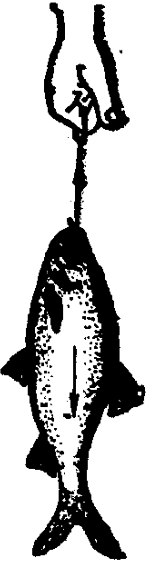
\includegraphics[width=1.5cm]{../pic/czwl1-ch2-16}
    \caption{}\label{fig:2-16}
    \end{minipage}
    \qquad
    \begin{minipage}{7cm}
    \centering
    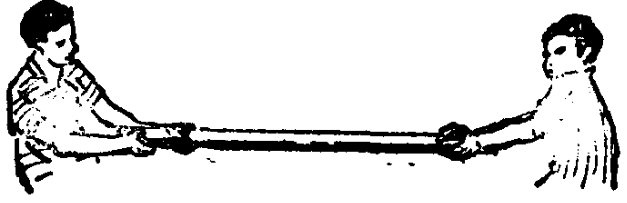
\includegraphics[width=7cm]{../pic/czwl1-ch2-17}
    \caption{}\label{fig:2-17}
    \end{minipage}
\end{figure}


作用在物体上的两个力在什么条件下才能够平衡呢?让我们来做图 \ref{fig:2-18} 所示的实验。
在小车的两端挂上细绳,细绳跨过滑轮,下端各吊一个小盘,两个小盘的质量相等。盘里放砝码。
小车受到两根细绳的方向相反的拉力 $F_1$ 和 $F_2$, 而且 $F_1$ 和 $F_2$ 在同一直线上。
实验表明,当两个盘里的砝码重相等,也就是 $F_1$ 和 $F_2$ 大小相等的时候,小车保持静止。
可见,\textbf{作用在一个物体上的两个力,如果在同一直线上,大小相等,方向相反,这两个力就平衡}。
两人拉一根棍子时,两人对棍子的拉力都沿着棍子,而且方向相反,如果两人的拉力大小相等,两个力就彼此平衡,这时棍子就保持静止不动。

\begin{figure}[htbp]
    \centering
    \begin{minipage}{7cm}
    \centering
    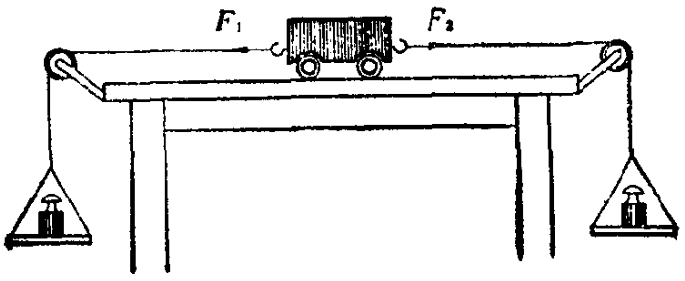
\includegraphics[width=6cm]{../pic/czwl1-ch2-18}
    \caption{}\label{fig:2-18}
    \end{minipage}
    \qquad
    \begin{minipage}{2cm}
    \centering
    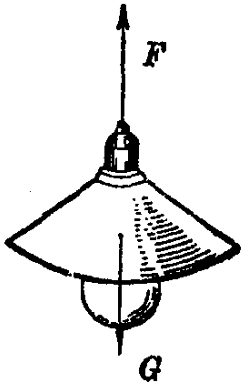
\includegraphics[width=2cm]{../pic/czwl1-ch2-19}
    \caption{}\label{fig:2-19}
    \end{minipage}
\end{figure}

一个物体在两个力作用下保持静止的现象,在日常生活中到处可以看到。
吊在电线上不动的电灯,受到两个力的作用,一个是向下的重力,一个是电线对它的向上的拉力,这两个力彼此平衡,所以电灯保持静止状态〈图 \ref{fig:2-19})。
放在桌子上静止不动的书,墨水瓶,一方面受到向下的重力,同时又受到桌子对它们向上的支持力,这两个力彼此平衡,所以书、墨水瓶保持静止状态。
放在地面上不动的箱子,也是在两个力的作用下保持静止状态的,它受到是哪两个力?请同学们自己分析一下。


\lianxi

(1) 挂在弹簧上的钩码静止不动时,钩码受到哪两个力的作用?这两个力的关系怎样?

(2) 你站在地面上静止不动时,身体受到哪两个力的作用?这两个力有什么关系?

(3) 茶杯重 2 牛顿,放在桌子上静止不动,茶杯受到哪两个力的作用?这两个力各是多大?方向怎样?用力的图示法画出茶杯所受的力来。

(4) 起重机钢丝绳上吊着的货物,在空中静止不动时,货物受到哪两个力的作用?它们的大小和方向怎样?
如果所吊的货物的质量是 5 吨, 这时钢丝绳对货物的拉力是多大?用力的图示法画出货物所受的力来。

(5) 作用在一个物体上的两个力分别如图 \ref{fig:2-20} 所示,这两个力能平衡吗?

\begin{figure}[htbp]
    \centering
    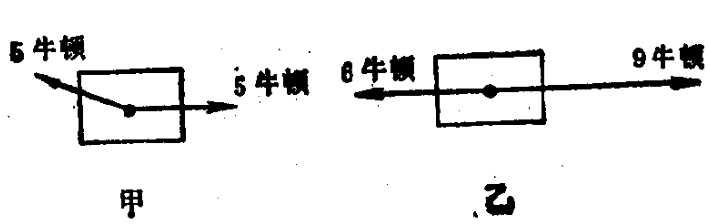
\includegraphics[width=0.6\textwidth]{../pic/czwl1-ch2-20}
    \caption{}\label{fig:2-20}
\end{figure}

\nonumsection{小实验:求形状不规则的物体的重心}

前面讲了几种形状规则的物体的重心。对于形状不规则的物体的重心,可以用下面的简单的实验方法求出来。
象图 \ref{fig:2-21} 那样,先通过物体上的任一点 $A$ 用绳子把物体挂起来。
当物体静止时,根据二力平衡的条件可以知道,物体受到的重力一定跟绳子的拉力在同一条直线上。
也就是说,物体的重心一定在通过 $A$ 点的竖直线上。用铅笔沿绳子在物体上画出竖直线 $AB$。
再通过另一点 $D$ 用绳子把物体悬挂起来,当物体静止时,同样可以知道,物体的重心一定在通过 $D$ 点的竖直线 $DE$ 上。
既然重心在直线 $AB$ 上,又在直线 $DE$ 上,所以,$AB$ 和 $DE$ 的交点 $C$ 就是物体的重心。
同学们可以用上面的方法来求出一块形状不规则的硬纸板的重心。

\begin{figure}[htbp]
    \centering
    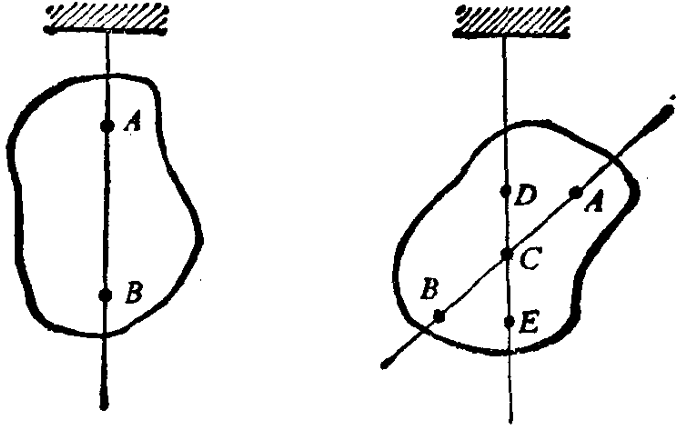
\includegraphics[width=0.6\textwidth]{../pic/czwl1-ch2-21}
    \caption{}\label{fig:2-21}
\end{figure}

为了验证 $C$ 点是纸板的重心,我们可以在纸板上任意另选一点 $M$, 通过 $M$ 点用绳子把纸板挂起来,
画出通过点 $M$ 的竖直线 $MN$,那么,$MN$ 也应该通过重心 $C$ 点。大家做一做,看看是不是这样。







